% !TeX root = RJwrapper.tex
\title{stppSim - An R Package For Synthesizing Spatiotemporal Point
Patterns}
\author{by Monsuru Adepeju}

\maketitle

\abstract{%
An abstract of less than 150 words.
}

\hypertarget{introduction}{%
\subsection{Introduction}\label{introduction}}

Introductory section which may include references in parentheses
\citep{R}, or cite a reference such as \citet{R} in the text.

\hypertarget{section-title-in-sentence-case}{%
\subsection{Section title in sentence
case}\label{section-title-in-sentence-case}}

This section may contain a figure such as Figure \ref{fig:Rlogo}.

\begin{Schunk}
\begin{figure}[htbp]

{\centering 
\includegraphics[width=2in]{Rlogo} 

}

\caption[The logo of R]{The logo of R.}\label{fig:Rlogo}
\end{figure}
\end{Schunk}

\hypertarget{another-section}{%
\subsection{Another section}\label{another-section}}

There will likely be several sections, perhaps including code snippets,
such as:

\begin{Schunk}
\begin{Sinput}
x <- 1:10
plot(x)
\end{Sinput}

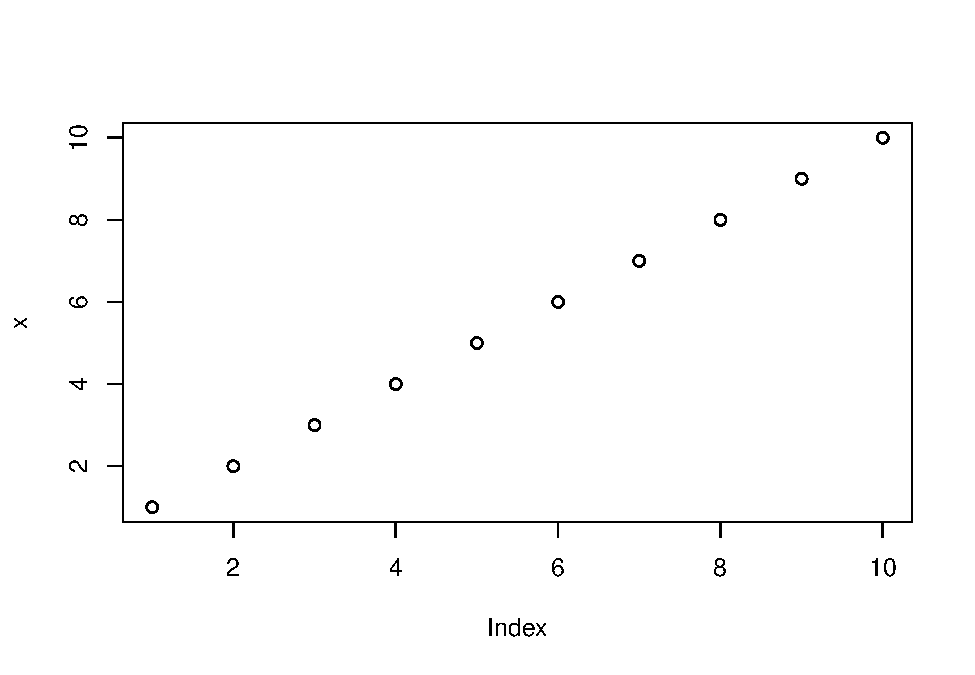
\includegraphics{RJtemplate_files/figure-latex/unnamed-chunk-1-1} \end{Schunk}

\hypertarget{summary}{%
\subsection{Summary}\label{summary}}

This file is only a basic article template. For full details of
\emph{The R Journal} style and information on how to prepare your
article for submission, see the
\href{https://journal.r-project.org/share/author-guide.pdf}{Instructions
for Authors}.

\hypertarget{about-this-format-and-the-r-journal-requirements}{%
\subsubsection{About this format and the R Journal
requirements}\label{about-this-format-and-the-r-journal-requirements}}

\texttt{rticles::rjournal\_article} will help you build the correct
files requirements:

\begin{itemize}
\tightlist
\item
  A R file will be generated automatically using \texttt{knitr::purl} -
  see \url{https://bookdown.org/yihui/rmarkdown-cookbook/purl.html} for
  more information.
\item
  A tex file will be generated from this Rmd file and correctly included
  in \texttt{RJwapper.tex} as expected to build \texttt{RJwrapper.pdf}.
\item
  All figure files will be kept in the default rmarkdown
  \texttt{*\_files} folder. This happens because
  \texttt{keep\_tex\ =\ TRUE} by default in
  \texttt{rticles::rjournal\_article}
\item
  Only the bib filename is to modifed. An example bib file is included
  in the template (\texttt{RJreferences.bib}) and you will have to name
  your bib file as the tex, R, and pdf files.
\end{itemize}

\bibliography{RJreferences.bib}

\address{%
Monsuru Adepeju\\
Crime and Well-Being Big Data Centre, Manchester Metropolitan
University\\%
All Saints Building, Manchester, M15 6BH\\ United Kingdom\\
%
\url{https://www.mmu.ac.uk}\\%
\textit{ORCiD: \href{https://orcid.org/0000-0002-9006-4934}{0000-0002-9006-4934}}\\%
\href{mailto:m.adepeju@mmu.ac.uk}{\nolinkurl{m.adepeju@mmu.ac.uk}}%
}
